\section*{}
\begin{figure}[h]
    \centering
    \begin{subfigure}[t]{0.49\textwidth}
        \centering
        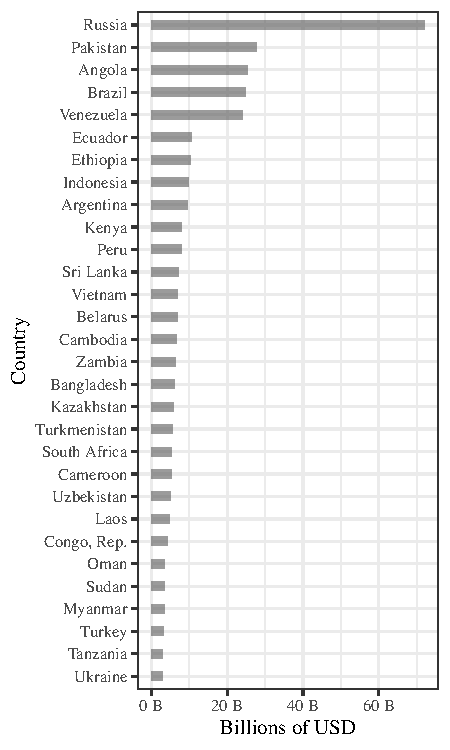
\includegraphics[width = \textwidth]{fig/total_debt.pdf}
        \caption{Top 30 Debtor by Total Debt in USD}
        \label{fig:total-debt-30}
    \end{subfigure}%
    ~
    \begin{subfigure}[t]{0.49\textwidth}
        \centering
        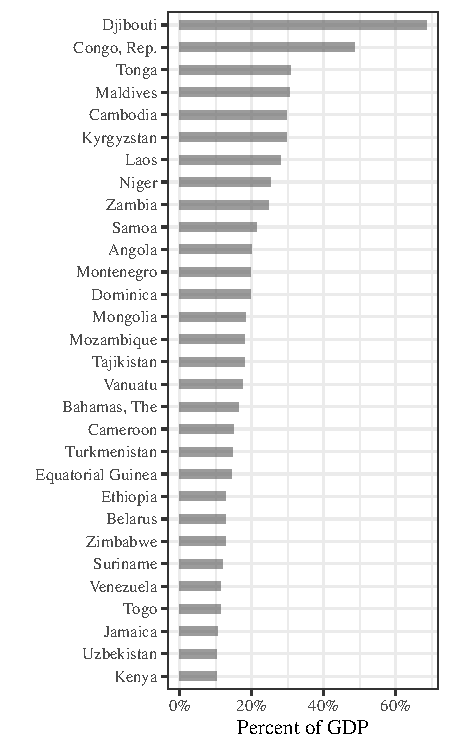
\includegraphics[width = \textwidth]{fig/perc_debt.pdf}
        \caption{Top 30 Debtor by Dept-to-GDP Ratio}
        \label{fig:perc-debt-30}
    \end{subfigure}
    \caption{Debt to China Statistic by Country in 2017}
    \label{fig:Country-Agg}
    \floatfoot{Source: \citet{Horn-Reinhart-Trebesch-21} database \\
    Note: The figure on the left presents the top 30 countries in amount of total external debt to China in 2017. The figure on the right compares by the China-debt-to-GDP ratio.}
\end{figure}

\begin{figure}[h]
    \centering
    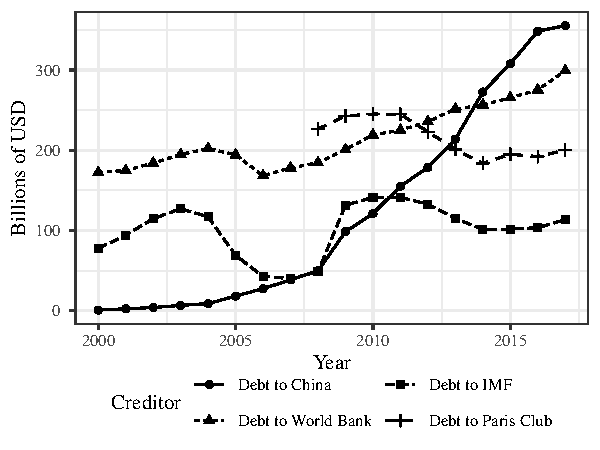
\includegraphics[width = 0.8\textwidth]{fig/aggr_debt_source.pdf}
    \caption{Change of Aggregate Public Debt for Different Official Creditors}
    \label{fig:debt-ts}
    \floatfoot{Source: \citet{Horn-Reinhart-Trebesch-21} database \\
    Note: The figure shows the change in the aggregate external public debt that the developing countries owed to different official creditors. These include China, World Bank (excluding China), IMF, and all 22 Paris Club governments. It is obvious that China had become the largest official creditors in the world according to the estimation of \citet*{Horn-Reinhart-Trebesch-21}.}
\end{figure}

\begin{figure}[h]
    \centering
    \begin{subfigure}[position]{0.8\textwidth}
        \centering
        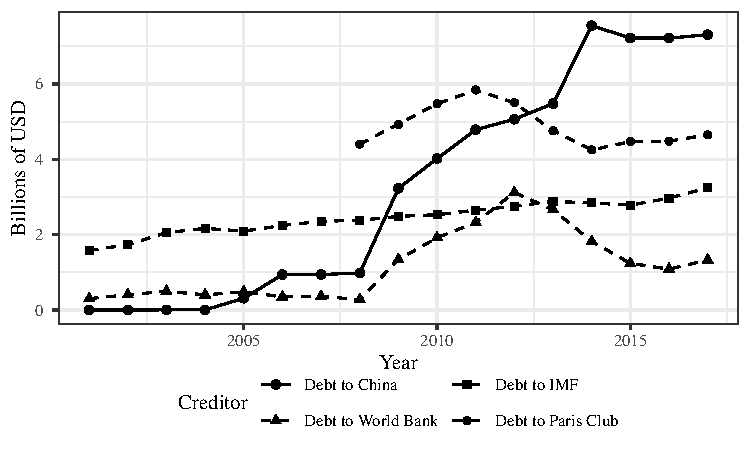
\includegraphics[width=\textwidth]{fig/ALL/Sri Lanka_debt_source.pdf}
        \caption{Sri Lanka}
        \label{fig: sri-lanka-debt-ts}
    \end{subfigure}
    \begin{subfigure}[position]{0.8\textwidth}
        \centering
        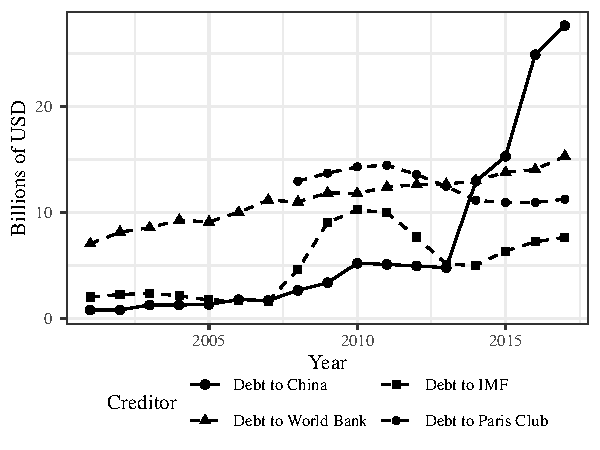
\includegraphics[width = \textwidth]{fig/ALL/Pakistan_debt_source.pdf}
        \caption{Pakistan}
        \label{fig: pakistan-debt-ts}
    \end{subfigure}
    \caption{Debt to Main Creditors}
    \label{fig: LAK-PAK-debt-ts}
    \floatfoot{Source: HRT Database \citeyearpar{Horn-Reinhart-Trebesch-21} \\
    Note: The figure shows the change in the external public debt that Sri Lanka and Pakistan owed to different official creditors. These include China, World Bank (excluding China), IMF, and all 22 Paris Club governments.}
\end{figure}

\begin{figure}[h]
    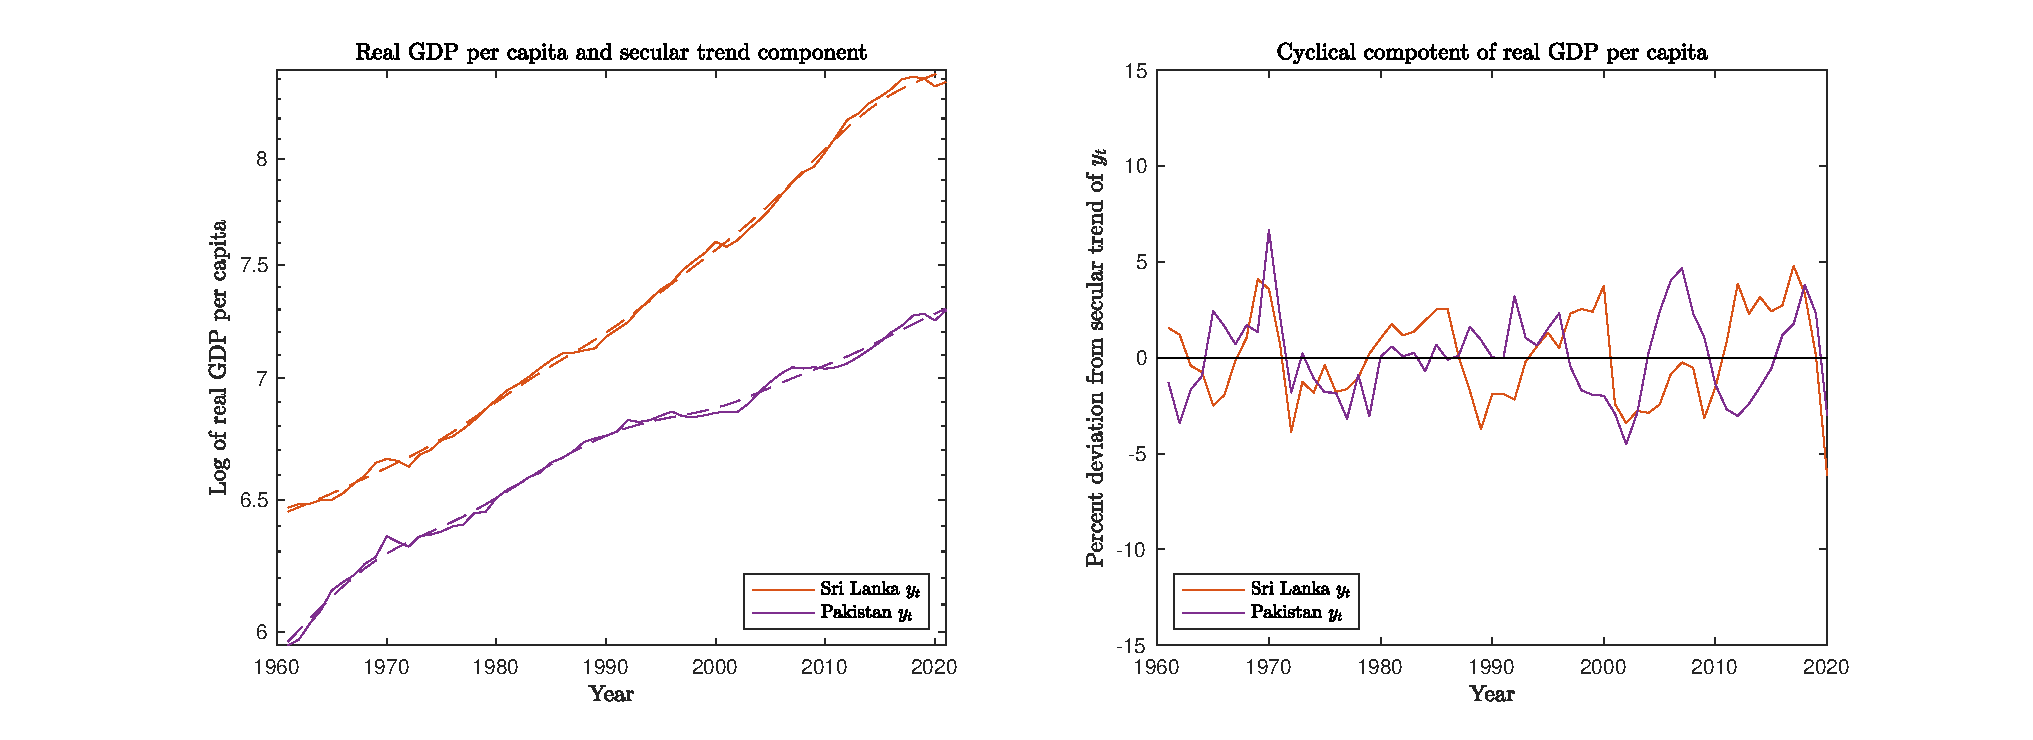
\includegraphics[width = \textwidth]{fig/decompose_gdp.eps}
    \caption{Decomposition of log-real-tradable-GDP for Sri Lanka and Pakistan}
    \label{fig:decompose-gdp}
    \floatfoot{\emph{Source:} World Bank national accounts data. \\
    \emph{Note:} The cyclical component in the right is obtained by the HP-filter with smoothing parameter $\lambda = 100$ for the log-real-GDP in the left. The quarterized AR(1) estimation for Sri Lanka yields $(\rho, \sigma_u)= (0.9114, 0.0123)$, and for Pakistan yields $(\rho, \sigma_u)= (0.9008, 0.0111)$}
\end{figure}
\section*{}

\begin{landscape}
    % Please add the following required packages to your document preamble:
% \usepackage{booktabs}
% \usepackage{graphicx}
\begin{table}[h]
    \centering
    % \footnotesize
    \begin{tabular}{@{}llll@{}}
    % \begin{tabular}{@{}lp{0.6\textwidth}lp{0.3\textwidth}@{}}
        \toprule
    Parameter  & Description                                                       & Value  & Source                                                                         \\ \midrule
    $\rho$     & Autocorrelation of output                                         & 0.9114  & Estimation of AR(1) on GDP\\
    $\sigma_u$ & Standard deviation of output                                      & 0.0123 & Estimation of AR(1) on GDP \\
    $r^*$      & Risk-free rate                                                    & 0.01 & U.S. 3-month treasury bill rate \\
    $\theta$   & Probability of reentry                                            & 0.0385 & \citet*{Chatterjee-12}                                              \\
    $\alpha$   & Labor share in non-tradable goods sector                          & 0.65   & \citet{Jegajeevan-Sri-Lanka-DSGE}                                                       \\
    $a$        & Share of tradable consumption                                     & 0.35   & Share of tradable goods in GPD                  \\
    $\xi$      & Intratemporal elasticity of substitution of consumption & 0.5   & \citet{Na-18}                             \\
    $\sigma$   & Inverse of intertemperal elasticity of substitution of consumption  & 2   & $1 / \xi$                                                                      \\
    $\beta$    & Discount factor                                                   & (\dots)  &  Self-estimated                                                                              \\
    $\delta_1$ & Coefficient of the linear term in loss function                   &  (\dots) &   Self-estimated                                                                             \\
    $\delta_2$ & Coefficient of the quadratic term in loss function                &  (\dots)   &               Self-estimated                                                                 \\
    $\bar{h}$  & Labor endowment                                                   & 1      & Normalized to 1\\
    \bottomrule
    \end{tabular}%
    \caption{Calibration for Sri Lanka}
    \label{tab:cal-sri-lanka}
    \floatfoot{\emph{Note}: The time unit is one quarter. AR(1) is performed on annual tradable GDP data but quarterized following the approach of \citet*{Hinrichsen_2020-chapter4}. }
    \end{table}
    % Please add the following required packages to your document preamble:
% \usepackage{booktabs}
% \usepackage{graphicx}
\begin{table}[h]
    \centering
    % \footnotesize
    \begin{tabular}{@{}llll@{}}
    % \begin{tabular}{@{}lp{0.6\textwidth}lp{0.3\textwidth}@{}}
        \toprule
    Parameter  & Description                                                       & Value  & Source                                                                         \\ \midrule
    $\rho$     & Autocorrelation of output                                         & 0.8518 & Estimation of AR(1) on GDP\\
    $\sigma_u$ & Standard deviation of output                                      & 0.0116 & Estimation of AR(1) on GDP\\
    $r^*$      & Risk-free rate                                                    & 0.01 & 3 month treasury bill rate \\
    $\theta$   & Probability of reentry                                            & 0.0417 & \citet*{trebesch-2011-sovereign}                                              \\
    $\alpha$   & Labor share in non-tradable goods sector                          & 0.4   & \citet{Pakistan-DSGE-calibration}                                                       \\
    $a$        & Share of tradable consumption                                     & 0.33   &Share of tradable goods in GDP                    \\
    $\xi$      & Intratemporal elasticity of substitution of consumption & 0.5   & \citet{Na-18}                              \\
    $\sigma$   & Inverse of intertemperal elasticity of substitution of consumption  & 2   & $1 / \xi$                                                                      \\
    $\gamma$   & Downward wage rigidity                                            & 1.048   & \citet*{wage-rigidity-data}                  \\
    $\beta$    & Discount factor                                                   & 0.6252  &  Estimated \\
    $\delta_1$ & Coefficient of the linear term in loss function                   &  -0.5148 &   Estimated  \\
    $\delta_2$ & Coefficient of the quadratic term in loss function                &  0.5789   &     Estimated   \\
    $\bar{h}$  & Labor endowment                                                   & 1      & Normalized to 1\\
    \bottomrule
    \end{tabular}%
    \caption{Calibration for Pakistan}
    \label{tab:cal-pakistan}
    \floatfoot{\emph{Note}: The time unit is one quarter. AR(1) is performed on annual tradable GDP data but quarterized following the approach of \citet*{Hinrichsen_2020-chapter4}. 
    ``Estimated'' means that the coefficient is obtained by matching certain equilibrium conditions, described in detail in Section \ref{sec: calibration}.}
    \end{table}
\end{landscape}